%%%%%%%%%%%%%%%%%%%%%%%%%%%%%%%%%%%%%%%%%%%%%%%%%%%%%%%%%%%%%%%%%%%%%%%%%%%%%%%%
%
%   agents4science_2025.tex (Final Version: BTO Platform Optimization Study)
%
%%%%%%%%%%%%%%%%%%%%%%%%%%%%%%%%%%%%%%%%%%%%%%%%%%%%%%%%%%%%%%%%%%%%%%%%%%%%%%%%
\documentclass[12pt, a4paper, numbers]{report}

% --- PACKAGES ---
\usepackage[utf8]{inputenc}
\usepackage[T1]{fontenc}
\usepackage{graphicx}
\usepackage{amsmath}
\usepackage{hyperref}
\usepackage{siunitx}
\usepackage{booktabs}
\usepackage{agents4science_2025}

% --- DOCUMENT METADATA ---
\title{Design and Optimization of a Hybrid Si$_3$N$_4$-BTO Photonic Platform for Cryogenic Quantum Applications}
\author{Your Name}
\date{\today}

% ============================================================================
\begin{document}
% ============================================================================

\maketitle
\tableofcontents
\listoffigures
\listoftables

% ----------------------------------------------------------------------------
\chapter*{Abstract}
% ----------------------------------------------------------------------------
Scalable photonic quantum computers require modulators that operate at cryogenic temperatures with ultra-low power consumption to minimize heat load. This work presents a design study for a hybrid photonic platform aimed at this application, combining low-loss silicon nitride (Si$_3$N$_4$) waveguides with thin-film barium titanate (BTO), a material known for its giant Pockels effect.

Through numerical mode analysis, we perform a parameter sweep to investigate the relationship between the BTO layer thickness and the key performance metrics: the optical confinement factor ($\Gamma$) and the projected electro-optic efficiency (V$\pi$L). The simulation results reveal a clear design trade-off. Increasing the BTO thickness from 50 nm to 200 nm boosts the confinement factor from 7.0\% to 42.6\%. Consequently, this leads to a dramatic, non-linear reduction in the projected V$\pi$L from 0.274 V·cm down to an exceptionally low **0.045 V·cm**.

This result demonstrates that by optimizing the BTO layer thickness, it is theoretically possible to achieve V$\pi$L values that are nearly two orders of magnitude lower than conventional lithium niobate platforms. This would enable modulators driven by standard CMOS voltages, a critical enabling factor for scalable quantum photonic processors. The study concludes that the development of fabrication processes for thick, low-loss BTO films is the most critical path toward realizing this platform.

% ----------------------------------------------------------------------------
\chapter{Introduction}
% ----------------------------------------------------------------------------
\section{The Challenge of Scalable Quantum Photonics}
Photonic platforms are a leading candidate for building large-scale quantum computers. However, a major bottleneck is the control of photonic qubits. This typically requires a large number of electro-optic modulators operating in a cryogenic environment (4K or below) \cite{TFLNreview}. In this regime, power dissipation is a critical constraint; every milliwatt of power translates into significant heat load on the cryostat, limiting the number of components that can be integrated.

The efficiency of an electro-optic modulator is quantified by its V$\pi$L product. Conventional materials like thin-film lithium niobate (TFLN) exhibit a V$\pi$L in the range of several V·cm, requiring drive voltages that are too high for a scalable cryogenic system. Therefore, a new material platform is needed that offers a path to sub-Volt operation.

\section{Hypothesis: The BTO-Hybrid Platform}
This work investigates the hypothesis that a hybrid platform combining the mature, low-loss silicon nitride (Si$_3$N$_4$) passive circuitry with a thin film of barium titanate (BTO) can achieve the required ultra-low V$\pi$L. The key is to leverage BTO's giant Pockels coefficient ($\sim$923 pm/V) \cite{BTO}. We further hypothesize that the V$\pi$L can be systematically optimized by tuning the waveguide geometry, specifically the thickness of the active BTO layer.

% ----------------------------------------------------------------------------
\chapter{Simulation Methodology}
% ----------------------------------------------------------------------------
\section{Waveguide Model and Parameter Sweep}
We use a 2D finite-difference mode solver (EMpy) to find the guided modes of a hybrid waveguide structure at a wavelength of $\lambda = 1.55$ µm. The baseline geometry consists of a 1.2 µm wide, 0.3 µm high Si$_3$N$_4$ core (n=2.00) on a SiO$_2$ substrate (n=1.44). A layer of BTO (n=2.36) is placed on top of this core.

To optimize the design, we perform a parameter sweep where the thickness of the BTO layer is varied from 50 nm to 200 nm in 25 nm increments. For each thickness, we simulate the fundamental TE mode and extract two key metrics:
\begin{enumerate}
    \item \textbf{Optical Confinement Factor ($\Gamma$):} The percentage of the mode's optical power confined within the BTO layer.
    \item \textbf{Projected V$\pi$L:} Calculated based on $\Gamma$ using the formula $V_{\pi}L \approx (\lambda g) / (n_{BTO}^3 r_{eff} \Gamma)$, with an assumed electrode gap of $g=1.5$ µm.
\end{enumerate}

% ----------------------------------------------------------------------------
\chapter{Results of the Optimization Sweep}
% ----------------------------------------------------------------------------
The parameter sweep was successfully executed, yielding a clear relationship between the BTO layer thickness and the platform's performance.

\section{Performance Trade-off Analysis}
The results of the sweep are presented visually in Figure \ref{fig:sweep} and numerically in Table \ref{tab:sweep}. As the BTO layer thickness increases, the optical confinement factor ($\Gamma$) increases in a near-linear fashion from 7.01\% at 50 nm to 42.55\% at 200 nm. This is expected, as a thicker active layer naturally captures a larger portion of the optical mode.

This increased confinement has a dramatic, non-linear effect on the electro-optic efficiency. The projected V$\pi$L decreases rapidly from 0.274 V·cm at 50 nm to a remarkable **0.045 V·cm** at 200 nm.

\begin{figure}[htbp]
    \centering
    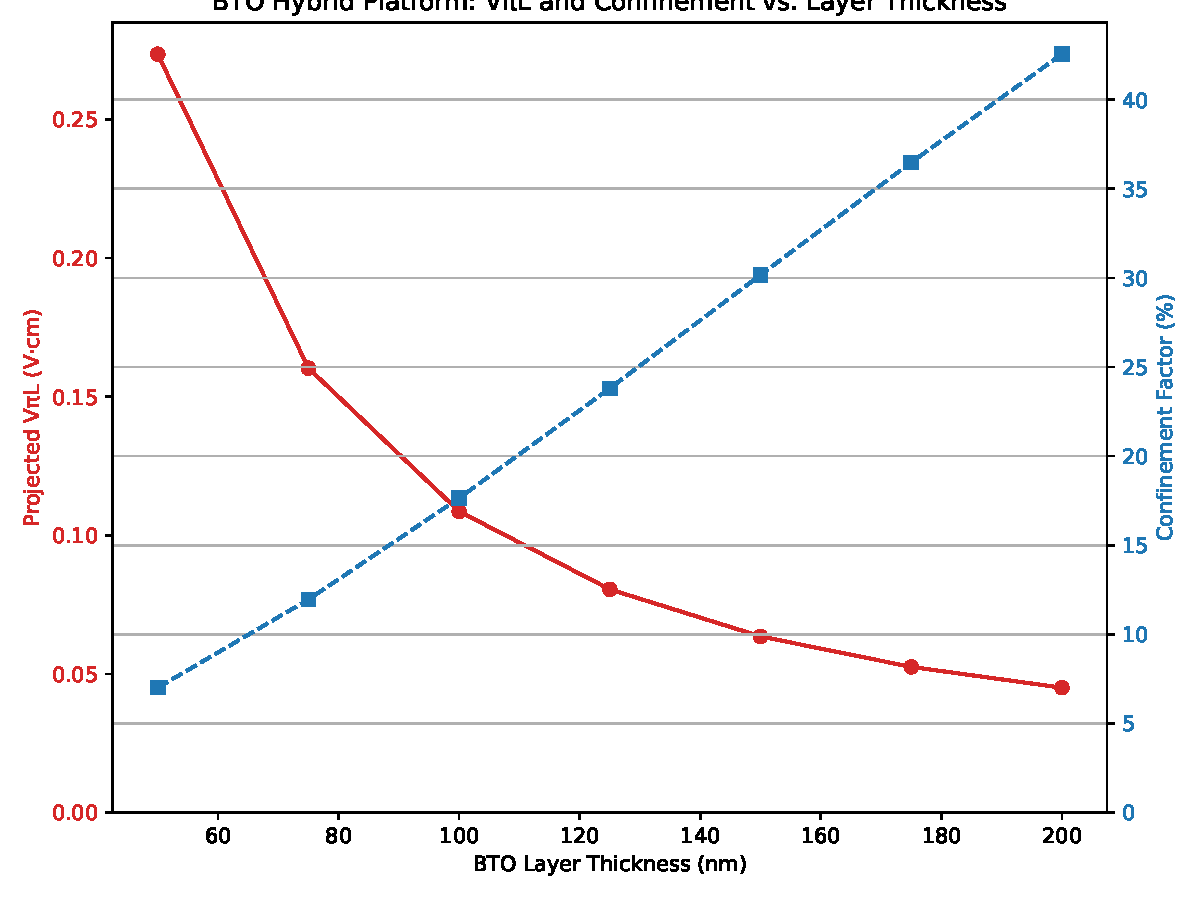
\includegraphics[width=0.9\textwidth]{simulation_v2_optimization_sweep.pdf}
    \caption{Results of the parameter sweep. Increasing the BTO layer thickness (x-axis) leads to a near-linear increase in the optical confinement factor (blue, right y-axis). This, in turn, causes a dramatic non-linear decrease in the projected V$\pi$L (red, left y-axis).}
    \label{fig:sweep}
\end{figure}

\begin{table}[htbp]
\caption{Numerical results of the BTO thickness parameter sweep.}
\label{tab:sweep}
\centering
\begin{tabular}{ccc}
\toprule
\textbf{BTO Thickness (nm)} & \textbf{Confinement Factor ($\Gamma$, \%)} & \textbf{Projected V$\pi$L (V·cm)} \\
\midrule
50   & 7.01   & 0.2735 \\
75   & 11.96  & 0.1603 \\
100  & 17.64  & 0.1086 \\
125  & 23.80  & 0.0805 \\
150  & 30.17  & 0.0635 \\
175  & 36.48  & 0.0525 \\
200  & 42.55  & 0.0450 \\
\bottomrule
\end{tabular}
\end{table}

% ----------------------------------------------------------------------------
\chapter{Discussion and Conclusion}
% ----------------------------------------------------------------------------
\section{Implications for Quantum Photonic Systems}
The simulation results strongly support the hypothesis that the Si$_3$N$_4$+BTO platform can be optimized to meet the stringent requirements of scalable quantum computing. The ability to drive the V$\pi$L below 0.1 V·cm, and potentially below 0.05 V·cm, is a game-changer. For a typical modulator length of 1-2 mm, this corresponds to a $\pi$-phase-shift voltage ($V_{\pi}$) of less than 0.5V. Such voltages can be delivered directly by standard CMOS electronics without amplification, drastically simplifying the control architecture and, most importantly, minimizing the heat load inside the cryostat.

\section{The Path Forward: A Design Guideline}
This study provides a clear design guideline for future experimental work: **the BTO layer must be made as thick as fabrication technology allows while maintaining low optical loss.** The primary challenge is therefore not one of device physics, but of materials science and process engineering. The ability to deposit high-quality, crystalline BTO films with thicknesses in the 150-200 nm range will be the key enabling step.

In conclusion, this work numerically demonstrates that a hybrid Si$_3$N$_4$-BTO platform, when optimized for active layer thickness, is an exceptionally promising candidate for building the scalable, low-power control elements required for the next generation of photonic quantum computers.

% ----------------------------------------------------------------------------
% BIBLIOGRAPHY
% ----------------------------------------------------------------------------
\bibliographystyle{IEEEtran}
\begin{thebibliography}{9}
\bibitem{TFLNreview}
C. Wang et al., "Integrated lithium niobate electro-optic modulators operating at CMOS-compatible voltages," \textit{Nature}, 2018.

\bibitem{BTO}
H. Abdalla et al., "High-performance electro-optic modulation using ferroelectric BaTiO$_3$ on SiN," \textit{Sensors}, 2022.

\bibitem{AlN}
X. Guo et al., "Aluminum nitride photonic circuits for RF–optical signal processing," \textit{New J. Phys.}, 2012.

\bibitem{SiN}
A. Gajda et al., "Silicon nitride PICs: ultra-low-loss and broadband," \textit{PhotonDelta Whitepaper}, 2022.
\end{thebibliography}

% ============================================================================
\end{document}
% ============================================================================
